\documentclass[UTF8]{gapd}

\Type{Article}


% !!为了公式敲入方便,额外引入amsmath包!!
\usepackage{amsmath}
\usepackage{float}
\Title{
  永不沉没的圆盘
}

\CAuthor{Ezio Sweet J. Ding}{华中科技大学物理实验创新基地}
\Author{Ezio Sweet J. Ding }{}

\Abstract{本文对IYPT2022年Unsinkable Disc进行理论、实验方面的简述}
\Keywords{水跃,流体力学}
%编号与页码(以下两行不需要改动)
\Issue{1}{1}{2022}
\Pages{1}{3}%37
\begin{document}
%\begin{CJK}{UTF8}{gbsn}
\maketitle

%一些常用的Latex语句:
%插入斜体:\textit{}
%引用文字:\begin{quote} \end{quote}
%插入脚标: \footnote{}

\section{简介}
\label{sec:unsinkable_disc_introduction}
根据人们的普遍印象,我们将一个金属圆盘浸没水中释放,圆盘自然会沉入水底,如果我们再在上面给它一个水流的冲击,根据我们的印象,自然沉入的更快,但是,有没有一种可能,添加了一个水的冲击,反而会使圆盘不沉没呢?

在下文中,我们就会讨论这个水流的冲击,到底会对圆盘造成什么。

\section{题目回顾}
\label{sec:unsinkable_disc_title_review}
A metal disk with a \textcolor{red}{hole} at its centre \textcolor{red}{sinks} in a container \textcolor{red}{filled with water}. When a \textcolor{red}{vertical} water jet hits the \textcolor{red}{centre} of the disc, it may \textcolor{red}{float on the water surface}. Explain this phenomenon and investigate the relevant parameters.

回顾题目,我们能够得到以下关键信息:
% !!这个模板中对于itemize的间距设置过大,建议后续进行一个调整!!
\begin{itemize}
    \item 实验对象:中间开孔的圆盘
    \item 实验环境:装满水的容器
    \item 实验操作:将水垂直射到圆盘的最中心
    \item 实验结果:圆盘漂浮在水面上
    \item 实验结论:得到相应的参数
\end{itemize}

根据题目思考,可以控制以下变量:
\begin{itemize}
    \item 圆盘的厚度、半价、孔半价、密度···
    \item 水流孔径、流速、流量···
\end{itemize}

也就是说,我们要总的研究分两部分,即圆盘和水流
%插入普通图片
\iffalse
\begin{figure}[!htbp]%
  \centering
  \includegraphics[width=0.8\columnwidth]{图片地址}
  \caption{图片名}
  \label{fig:P2}%\label置于\caption后,否则可能报错
\end{figure}
\fi%实际写时不需要\iffalse \fi,(该组命令是为了编辑时不报错)

%插入跨列图片
\iffalse
\begin{figure*}[!htbp]
  \centering
  \includegraphics[width=1\linewidth]{图片地址}
  \caption{图片名}
  \label{fig:P1}
\end{figure*}
\fi

%插入图表一定要注意规范!!!!!!!!!!!!!!!!!!!!!!!!!!!!!!!!!!!!!!
%表格一律用三线表,如果有出现数据,请注明数据的单位,另外表格的标题等也要注明清楚。

%插入任何非原创图片都应当注意注明出处
%插入一般的曲线图,一定要注明坐标轴的含义!!!!!及其单位!!!!!!  格式一律为:      物理量 (单位)
%                                                                              ^
%                                                                              |
%                                                                              |
%                                                                              |
%                                                                例子:         ——————————————————————————>
%                                                                                     摆线长度  (mm)
%当图中存在多个曲线,或者数据与拟合图同时存在时,要写清楚图例!!!!!!!!!
%要善于运用跨列图片,把多个相似的子图拼组合成一张比较大的跨列图片


\section{理论}
\label{sec:unsinkable_disc_theory}
\subsection{假设}
\subsubsection{假设的提出}
\begin{enumerate}
    \item 水可以视作理想流体,水的黏性可以忽略不计
    \item 圆盘的上表面有水,表面张力忽略; 
    \item 高度一定时,同一次实验中水管中流出的水的流量是恒定的;
    \item 气泡对圆盘沉浮的影响可以忽略不计
\end{enumerate}

好的假设是构建优秀理论的前提,我们将目光放在影响更大的因素中,合理的划分研究范围,对于简化理论和提高实验可行度有很大帮助
\subsubsection{假设合理性验证}

\noindent .1  对实验条件下雷诺数的计算

雷诺数是表征流体流动的无量纲数,可以通过以下函数确定,其中$\rho$为液体密度,$v$为液体流速,$d$为特征长度,一般表现为内径,$\eta$为流体黏性系数。

由以下公式可得:

\begin{align}
    Re=\frac{\rho vd}{\eta}
\end{align}

在我们的实验条件中,有(置信概率为99.73\%)
\begin{align}
    &d=(14.70 \pm 0.21)\text{mm}\\
    &v=(0.81 \pm 0.01)\text{m/s}
\end{align}
\subsection{水跃现象}
水跃(Hydraulic jump)是流体力学的现象,常在像河或泄洪道的明渠中出现。当高流速的超临界流进入低流速的亚临界流中,流体的速度突然变慢,因此流体部分的动能被紊流消散,部分动能则转换为位能,造成液面明显变高,这样的现象即为水跃。\cite{wiki:水跃}

\begin{figure}[!htbp]%
  \centering
  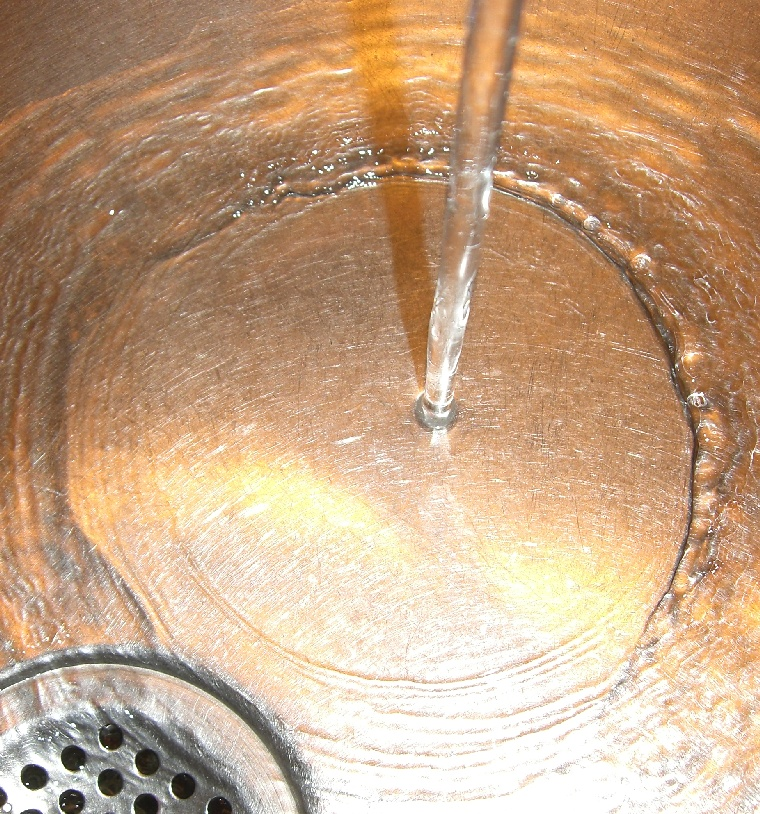
\includegraphics[width=0.8\columnwidth]{unsinkable_disc_src/images/shock_sink.jpg}
  \caption{水跃现象\cite{wiki:水跃}}
  \label{fig:unsinkable_disc_hudraulia_jump}%\label置于\caption后,否则可能报错
\end{figure}

水跃现象会对发生水跃的平面施加一个向上的力,这个力由下式确定:
\begin{align}
    F=\begin{cases}
        h_2\rho g \pi (r_p^2-r_k^2),r_1>r_p\\
        h_2\rho g \pi (r_1^2-r_k^2),r_1\le r_p
    \end{cases} \label{eq:unsinkable_disc_core}
\end{align}

其中$h_2$水跃后的高度,$\rho$为液体的密度,$g$ 为重力加速度,$r_1$  为水跃距离 , $r_p$ 为圆盘半径,$r_k$为孔的半径
\subsection{受力分析}

对圆盘进行受力分析,可得
\begin{figure}[!htbp]%
  \centering
  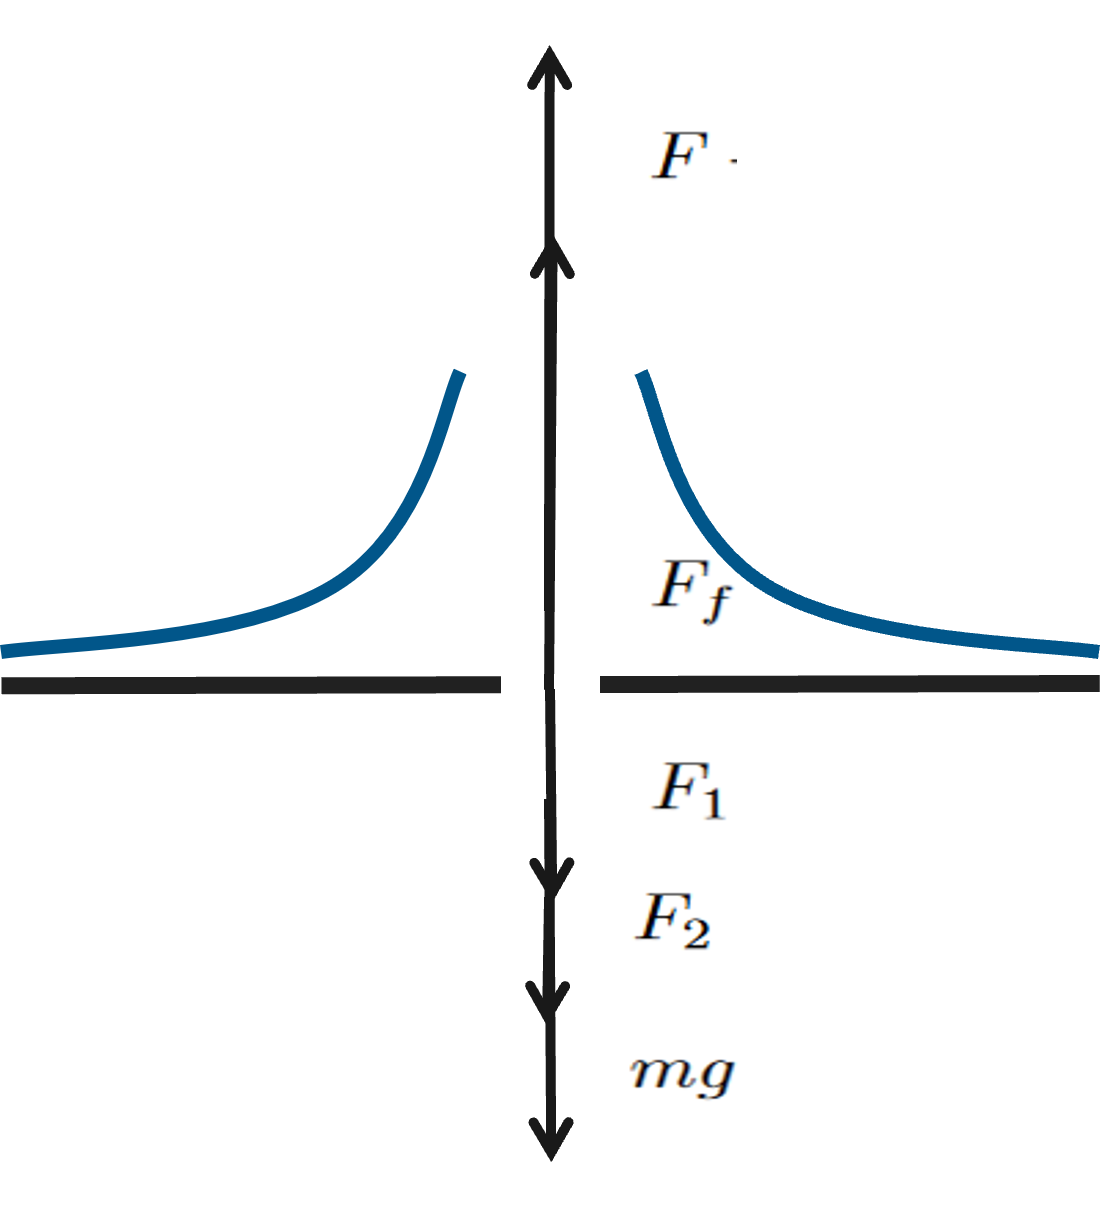
\includegraphics[width=0.8\columnwidth]{unsinkable_disc_src/images/f_analysis.png}
  \caption{受力分析} 
  \label{fig:unsinkable_disc_force_analysis}%\label置于\caption后,否则可能报错
\end{figure}

圆盘不沉没的条件为:
\begin{align}
    F+F_f\ge F_1+F_2+mg 
\end{align}

其中$F_1$为圆盘上水对圆盘的压力,$F_2$为水流对圆盘的冲击力
\subsection{盘上水质量的计算和冲击力的计算}
在进行实验时,我们控制水的流量恒定,则有:
\begin{align}
    F_1=\frac{Qr_p\rho g}{v}
\end{align}

其中 $v$ 为水在圆盘上的流动速度,由视频拆帧算得

由动量定理,可以得到:
\begin{align}
    F_2dt&=mu
    F_2&=\rho Q u
\end{align}

其中 $u$  为水冲击到圆盘上的速度,由视频拆帧算得
\subsection{水跃高度的计算}
由(1)(2)式可知,我们需要导出  $h_2$  ,我们可以运用由伯努利方程推出的水跃方程\cite{article:1}:
\begin{align}
    \frac{\beta \rho Q^2}{A_1}+\rho g h_{c1}A_1=\frac{\beta \rho Q^2}{A_2}+\rho g h_{c2}A_2
\end{align}

其中  $\beta$ 为动量校正系数,取决于水速度分布水在圆盘上的流动分布均匀程度,
$A_1$、$A_2$为跃前,跃后断面面积,有
\begin{align}
    A_1&=2\pi r_p h_1\\
    A_2&=2\pi(r_p+l)h_2
\end{align}

\noindent$l$为水跃长度,由经验公式得到(经验公式适用范围见参考文献\cite{book:1}):
\begin{align}
    l=10.8h_1(Fr-1)^{0.93}
\end{align}

\noindent$Fr$为弗劳德数,由下式计算\cite{article:2}:
\begin{align}
    Fr&=\frac{v}{\sqrt{g \bar{h}}}\\
    \bar{h}&=\frac{h_1+h_2}{2}
\end{align}

$h_{c1}$、$h_{c2}$为 $A_1,A_2$的形心点水深,由下式计算:
\begin{align}
    h_{ci}=\frac{h_i}{2},i=1,2
\end{align}

综上,代入\eqref{eq:unsinkable_disc_core}即可解出结果
\section{实验}
\label{sec:unsinkable_disc_experiment}
\subsection{实验步骤}
\begin{enumerate}
    \item 搭建装置,检查装置气密性
    \item 调节水流,使流量稳定
    \item 将圆盘微沉于水中,使用相机录制视频以便拆帧计算速度和流量
    \item 整理实验数据,画图,计算误差
\end{enumerate}
\subsection{实验装置及实验平台}
实验用到的圆盘如图\ref{fig:unsinkable_disc_discs}所示
\begin{figure}[H]%
  \centering
  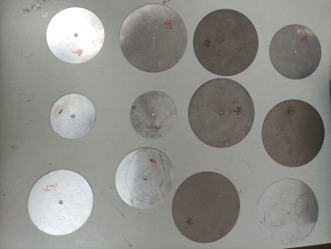
\includegraphics[width=0.8\columnwidth]{unsinkable_disc_src/images/disc.jpg}
  \caption{圆盘}
  \label{fig:unsinkable_disc_discs}%\label置于\caption后,否则可能报错
\end{figure}

圆盘的尺寸及不确定度如表格\ref{tab:unsinkable_disc_disc's_size}和\ref{tab:unsinkable_disc_disc's_uncertainty}所示
\begin{table*}[htbp]
    \centering
    \begin{tabular}{cccc}
        \hline
         圆盘序号&孔直径(mm)&圆盘直径(cm)&圆盘厚度(mm)\\
        \hline
         1&5.99&7.990&0.42\\
         2&/&8.452&0.41\\
         3&5.95&9.964&0.42\\
         4&6.00&11.409&0.42\\
         5&4.92&11.989&0.43\\
         6&3.04&9.992&0.49\\
         7&3.00&11.980&0.80\\
         8&3.01&11.977&0.32\\
         9&/&11.960&0.32\\
         \hline
    \end{tabular}
    \caption{圆盘尺寸}
    \label{tab:unsinkable_disc_disc's_size}
\end{table*}
\begin{table*}[htbp]
    \centering
    \begin{tabular}{cccc}
        \hline
         圆盘序号&孔直径不确定度(mm)&圆盘直径不确定度(cm)&圆盘厚度不确定度(mm)\\
        \hline
         1&0.02&0.012&0.02\\
         2&/&0.043&0.01\\
         3&0.05&0.054&0.02\\
         4&0.05&0.173&0.02\\
         5&0.07&0.012&0.02\\
         6&0.07&0.002&0.01\\
         7&0.01&0.066&0.01\\
         8&0.01&0.054&0.56\\
         9&/&0.009&0.56\\
         \hline
    \end{tabular}
    \caption{圆盘尺寸不确定度}
    \label{tab:unsinkable_disc_disc's_uncertainty}
\end{table*}

实验平台的搭建如图\ref{fig:unsinkable_disc_platform1}和\ref{fig:unsinkable_disc_platform2}所示
\begin{figure}[!htbp]%
  \centering
  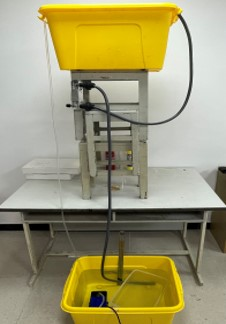
\includegraphics[width=0.8\columnwidth]{unsinkable_disc_src/images/platform1.jpg}
  \caption{实验室实验平台}
  \label{fig:unsinkable_disc_platform1}%\label置于\caption后,否则可能报错
\end{figure}

\begin{figure}[!htbp]%
  \centering
  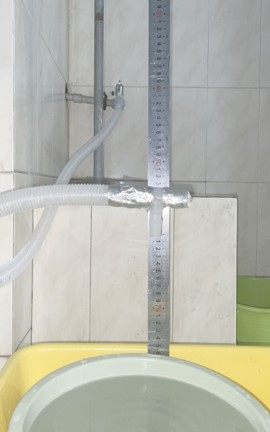
\includegraphics[width=0.8\columnwidth]{unsinkable_disc_src/images/platform2.jpg}
  \caption{室外实验平台}
  \label{fig:unsinkable_disc_platform2}%\label置于\caption后,否则可能报错
\end{figure}

\subsection{实验流程}
我们将实验区分为高流量组和低流量组两组
如图\ref{fig:unsinkable_disc_platform1}所示,我们利用重力提供水压,将水从上方的容器延水管射至下方,同时我们在下方的容器中设置一个水泵,将水源源不断的抽至上方的容器中,形成水的循环利用。

启动水泵,将水利用虹吸效应从上方吸下,冲击到圆盘的最中心,使圆盘漂浮在水面上。

在实验中,我们能够很明显的看出圆盘十分不稳定,很难控制水流一直射到圆盘的正中心,如何控制圆盘的位置不轻易改变是一个很大的难题。

起初我们打算使用一根铁丝从圆盘小孔略微穿出,使圆盘只能在这个环绕这个铁丝运动,但是在后续的实验中,我们发现,这样做会极大的削减水流击打在孔时的流速,对于实验产生了不可忽略的影响。

然后我们又试着使用铁丝编织一个铁架,将圆盘放在铁架中间,但是在水槽中,铁架的固定又成为一个问题,最终作罢。

在室外的实验中,我们放弃了重力产生流量的方式,原因在于无论怎么调整高度都难以在一层楼的高度里达到较大的流速,我们换用一个软管直接接水龙头,产生较快的流速,使用视频拆帧\cite{gh:SAE}的方式分析流速,得到较为合理的结果。

在实验中,我们设置了两个无孔圆盘,作为对比实验

实验图像如图\ref{fig:unsinkable_disc_experiment}所示
\begin{figure}[!htbp]%
  \centering
  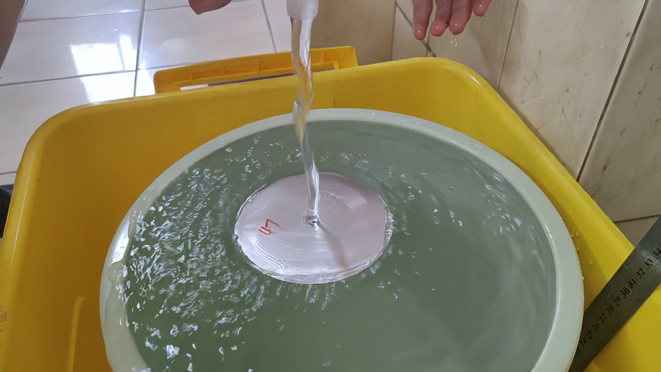
\includegraphics[width=0.8\columnwidth]{unsinkable_disc_src/images/experiment.png}
  \caption{实验图像}
  \label{fig:unsinkable_disc_experiment}%\label置于\caption后,否则可能报错
\end{figure}

经过实验,我们测得一系列数据,请访问\url{https://phys.eziosweet.cn/#/%E6%B0%B8%E4%B8%8D%E6%B2%89%E6%B2%A1%E7%9A%84%E5%9C%86%E7%9B%98/%E5%9C%86%E7%9B%98%E6%95%B0%E6%8D%AE}获得

\subsection{实验数据后处理}

以下是三组数据的可视化

蓝色点为浮点,红色点为沉点,线以上为理论上下沉,线以下为理论上上浮。
\begin{figure}[!htbp]%
  \centering
  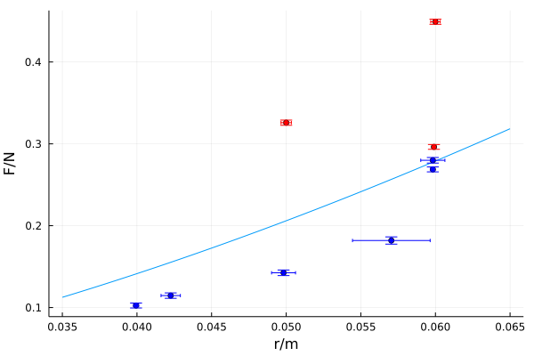
\includegraphics[width=0.8\columnwidth]{unsinkable_disc_src/images/36.5.png}
  \caption{$Q$=36.5ml}
  \label{fig:unsinkable_disc_36.5}%\label置于\caption后,否则可能报错
\end{figure}

\begin{figure}[!htbp]%
  \centering
  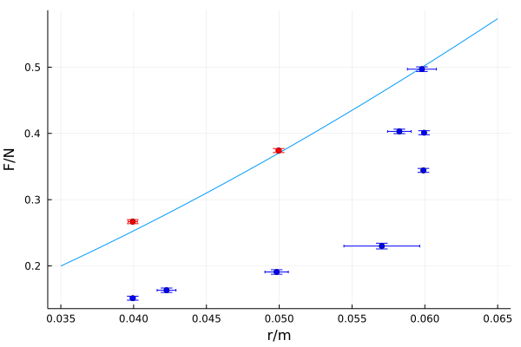
\includegraphics[width=0.8\columnwidth]{unsinkable_disc_src/images/68.7.png}
  \caption{$Q$=68.7ml}
  \label{fig:unsinkable_disc_68.7}%\label置于\caption后,否则可能报错
\end{figure}

\begin{figure}[!htbp]%
  \centering
  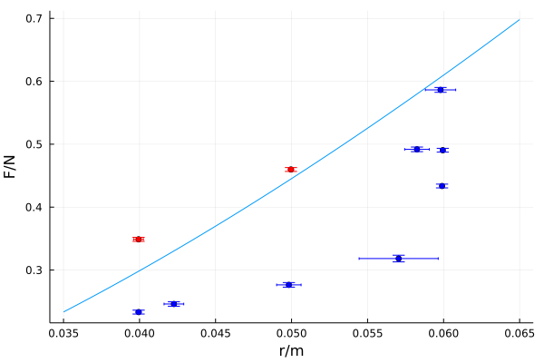
\includegraphics[width=0.8\columnwidth]{unsinkable_disc_src/images/99.0.png}
  \caption{$Q$=99.0ml}
  \label{fig:unsinkable_disc_99.0}%\label置于\caption后,否则可能报错
\end{figure}

由图可知,实验和理论拟合的很好,尽管存在一定误差,但基本验证了理论的正确性

\section{结果分析}
通过理论和实验的双重验证,我们认为影响圆盘浮沉的因素在于上升力和下降力的角逐。

上升力中主要为圆盘自身的浮力和水跃产生的压力,其中水跃产生的压力对上升起主要作用,影响水跃的因素有圆盘半径,孔半径和水流流量。

下降力中主要为圆盘自身的重力和圆盘上水的重力以及水流对于圆盘的冲击力,

\section{误差分析}
以下是我们想到的可能的误差来源:
\subsection{系统误差}
\begin{itemize}
    \item 实验中未考虑盘下气泡对实验产生的影响,尽管无孔圆盘的实验说明了气泡对实验没有太大的影响,但是仍旧存在系统误差。
    \item 实验中对流体做了无黏假设,但是实际上水仍旧存在一些黏性
\end{itemize}
\subsection{人员和仪器误差}
\begin{itemize}
    \item 实验中使用的游标卡尺的分度值为0.02mm,存在一定的示值误差
    \item 实验中使用视频拆帧计算瞬时速度,采用的帧率为59.94帧,将每两帧之间的平均速度作为瞬时速度
    \item 实验人员在实验过程中不可避免会产生一定的误差
\end{itemize}

\section{展望}
在我们划分的研究范围中,我们认为已经做的较好,但是仍旧有可以提升的空间
\subsection{气泡对实验的影响}
实验中并未对气泡进行详细的探究,在未来的实验中,我们打算深入对气泡的影响进行探究。
\subsection{波浪荷载}
在文献查阅的过程中,我们发现波浪荷载会对其中的物体产生力的作用,但是我们查阅的资料中均讨论的是波浪从一个方向向另一个方向运动,与我们的实验不符,在进一步的研究中,我们会探讨波浪荷载对实验是否会产生影响。
%致谢,参考文献与背景信息部分=========================================================
\section*{致谢}
感谢华中科技大学物理学院物理实验创新基地学长们、老师们、同学们在该实验中提供的帮助。

感谢@Justin62628开源的Squirrel Anime Enhance为我们进行简单的视频拆帧提供了可能

感谢Google Scholar提供的简单好用的文献搜索

感谢JetBrains提供的面向学生的免费IDE
%致谢部分记得改过来好吗!!!!仔细看看模板的内容!!!!!!!!!!!!!!!!!!

\section*{附录}
本实验使用的文献,得到的数据等资料均可在
\url{https://phys.eziosweet.cn/#/%E6%B0%B8%E4%B8%8D%E6%B2%89%E6%B2%A1%E7%9A%84%E5%9C%86%E7%9B%98}下载使用
%背景信息
\Note{BlueNoteBackground}{
  {\textbf{Author:}} Ezio Sweet J. Ding\\
  {\textbf{Address:}} School of Physics, Huazhong University of Science and Technology\\
  {\textbf{Email:}} eziosweet@ibpe.eu.org\\
  {\textbf{Blog:}} \url{https://blog.eziosweet.cn}\\
  {\textbf{PhysDrive:}} \url{https://phys.eziosweet.cn}
}
%写上你们的背景信息呀!!!!!!这上面的背景信息都是乱填的呀!!!!!!!!!!!
%觉得多余的可以删去,觉得不够的也可以增添别的背景信息!!!!!!!!!!!!!!!!!!!!!!!!!!!!
\section*{参考文献}
\bibliographystyle{amsplain}
\bibliography{unsinkable_disc_src/bibtex/unsinkable_disc}
% \section*{参考文献}
% \begin{thebibliography}{2}

% \bibitem{c1}Browne C. ,Deductive Search for Logic Puzzles,
% \textit{Computational Intelligence and Games (CIG'13)}, 
% IEEE Press,2013, pp.~359--366.

% \bibitem{c2}Higashida H.,Machine-Made Puzzles andHand-Made Puzzles, \textit{IFIP Advances in Information andCommunication Technology (AICT)}, vol.~333, 2010, pp. 214--222.

% \end{thebibliography}

%\end{CJK}
\end{document}
